% Options for packages loaded elsewhere
% Options for packages loaded elsewhere
\PassOptionsToPackage{unicode}{hyperref}
\PassOptionsToPackage{hyphens}{url}
%
\documentclass[
  ignorenonframetext,
  aspectratio=169,
  russian,
]{beamer}
\newif\ifbibliography
\usepackage{pgfpages}
\setbeamertemplate{caption}[numbered]
\setbeamertemplate{caption label separator}{: }
\setbeamercolor{caption name}{fg=normal text.fg}
\beamertemplatenavigationsymbolshorizontal
% remove section numbering
\setbeamertemplate{part page}{
  \centering
  \begin{beamercolorbox}[sep=16pt,center]{part title}
    \usebeamerfont{part title}\insertpart\par
  \end{beamercolorbox}
}
\setbeamertemplate{section page}{
  \centering
  \begin{beamercolorbox}[sep=12pt,center]{section title}
    \usebeamerfont{section title}\insertsection\par
  \end{beamercolorbox}
}
\setbeamertemplate{subsection page}{
  \centering
  \begin{beamercolorbox}[sep=8pt,center]{subsection title}
    \usebeamerfont{subsection title}\insertsubsection\par
  \end{beamercolorbox}
}
% Prevent slide breaks in the middle of a paragraph
\widowpenalties 1 10000
\raggedbottom
\AtBeginPart{
  \frame{\partpage}
}
\AtBeginSection{
  \ifbibliography
  \else
    \frame{\sectionpage}
  \fi
}
\AtBeginSubsection{
  \frame{\subsectionpage}
}
\usepackage{iftex}
\ifPDFTeX
  \usepackage[T1]{fontenc}
  \usepackage[utf8]{inputenc}
  \usepackage{textcomp} % provide euro and other symbols
\else % if luatex or xetex
  \usepackage{unicode-math} % this also loads fontspec
  \defaultfontfeatures{Scale=MatchLowercase}
  \defaultfontfeatures[\rmfamily]{Ligatures=TeX,Scale=1}
\fi
\usepackage{lmodern}

\usetheme[]{metropolis}
\ifPDFTeX\else
  % xetex/luatex font selection
\fi
% Use upquote if available, for straight quotes in verbatim environments
\IfFileExists{upquote.sty}{\usepackage{upquote}}{}
\IfFileExists{microtype.sty}{% use microtype if available
  \usepackage[]{microtype}
  \UseMicrotypeSet[protrusion]{basicmath} % disable protrusion for tt fonts
}{}


\usepackage{longtable,booktabs,array}
\usepackage{calc} % for calculating minipage widths
\usepackage{caption}
% Make caption package work with longtable
\makeatletter
\def\fnum@table{\tablename~\thetable}
\makeatother
\usepackage{graphicx}
\makeatletter
\newsavebox\pandoc@box
\newcommand*\pandocbounded[1]{% scales image to fit in text height/width
  \sbox\pandoc@box{#1}%
  \Gscale@div\@tempa{\textheight}{\dimexpr\ht\pandoc@box+\dp\pandoc@box\relax}%
  \Gscale@div\@tempb{\linewidth}{\wd\pandoc@box}%
  \ifdim\@tempb\p@<\@tempa\p@\let\@tempa\@tempb\fi% select the smaller of both
  \ifdim\@tempa\p@<\p@\scalebox{\@tempa}{\usebox\pandoc@box}%
  \else\usebox{\pandoc@box}%
  \fi%
}
% Set default figure placement to htbp
\def\fps@figure{htbp}
\makeatother



\ifLuaTeX
\usepackage[bidi=basic,provide=*]{babel}
\else
\usepackage[bidi=default,provide=*]{babel}
\fi
% get rid of language-specific shorthands (see #6817):
\let\LanguageShortHands\languageshorthands
\def\languageshorthands#1{}


\setlength{\emergencystretch}{3em} % prevent overfull lines

\providecommand{\tightlist}{%
  \setlength{\itemsep}{0pt}\setlength{\parskip}{0pt}}



 

\usepackage[]{csquotes}

\IfFileExists{plex-otf.sty}{
  %% Full TeXlive
  % \usepackage[%
  %   % math,
  %   RM={Scale=0.94},SS={Scale=0.94},SScon={Scale=0.94},TT={Scale=MatchLowercase,FakeStretch=0.9},DefaultFeatures={Ligatures=Common}
  % ]{plex-otf}
}{
  %% TinyTeX
  \usepackage{libertine}
}

%%% Load theme
% https://deic.uab.cat/~iblanes/beamer_gallery/
\IfFileExists{beamerthemegotham.sty}{
  %% Full TeXlive
  \usetheme{gotham}
  \gothamset{
    numbering=totalpagenumber,
    parttocframe default=off,
    sectiontocframe default=off,
    subsectiontocframe default=off,
  }
}{
  %% TinyTeX
  \usetheme{Madrid}
}
\makeatletter
\@ifpackageloaded{caption}{}{\usepackage{caption}}
\AtBeginDocument{%
\ifdefined\contentsname
  \renewcommand*\contentsname{Содержание}
\else
  \newcommand\contentsname{Содержание}
\fi
\ifdefined\listfigurename
  \renewcommand*\listfigurename{Список иллюстраций}
\else
  \newcommand\listfigurename{Список иллюстраций}
\fi
\ifdefined\listtablename
  \renewcommand*\listtablename{Список таблиц}
\else
  \newcommand\listtablename{Список таблиц}
\fi
\ifdefined\figurename
  \renewcommand*\figurename{Рисунок}
\else
  \newcommand\figurename{Рисунок}
\fi
\ifdefined\tablename
  \renewcommand*\tablename{Таблица}
\else
  \newcommand\tablename{Таблица}
\fi
}
\@ifpackageloaded{float}{}{\usepackage{float}}
\floatstyle{ruled}
\@ifundefined{c@chapter}{\newfloat{codelisting}{h}{lop}}{\newfloat{codelisting}{h}{lop}[chapter]}
\floatname{codelisting}{Список}
\newcommand*\listoflistings{\listof{codelisting}{Листинги}}
\makeatother
\makeatletter
\makeatother
\makeatletter
\@ifpackageloaded{caption}{}{\usepackage{caption}}
\@ifpackageloaded{subcaption}{}{\usepackage{subcaption}}
\makeatother

\usepackage{bookmark}
\IfFileExists{xurl.sty}{\usepackage{xurl}}{} % add URL line breaks if available
\urlstyle{same}
\hypersetup{
  pdftitle={Лабораторная работа № 2},
  pdfauthor={Александр Прядко},
  pdflang={ru-RU},
  hidelinks,
  pdfcreator={LaTeX via pandoc}}


\title{Лабораторная работа № 2}
\subtitle{Дискреционное разграничение прав в Linux. Основные атрибуты}
\author{Александр Прядко}
\date{2026-03-07}

\begin{document}
\frame{\titlepage}

\renewcommand*\contentsname{Содержание}
\begin{frame}[allowframebreaks]
  \frametitle{Содержание}
  \setcounter{tocdepth}{1}
  \tableofcontents
\end{frame}
\setcounter{tocdepth}{1}
\tableofcontents
}

\section{Информация}\label{ux438ux43dux444ux43eux440ux43cux430ux446ux438ux44f}

\begin{frame}{Докладчик}
\phantomsection\label{ux434ux43eux43aux43bux430ux434ux447ux438ux43a}
\begin{itemize}[<+->]
\tightlist
\item
  \textbf{Александр Прядко}
\item
  Студент кафедры кибербезопасности
\item
  Российский университет дружбы народов им. П. Лумумбы
\item
  Дисциплина: Информационная безопасность
\item
  \href{mailto:alex-pryadko@example.com}{\nolinkurl{alex-pryadko@example.com}}
\end{itemize}
\end{frame}

\section{Вводная
часть}\label{ux432ux432ux43eux434ux43dux430ux44f-ux447ux430ux441ux442ux44c}

\begin{frame}{Цель работы}
\phantomsection\label{ux446ux435ux43bux44c-ux440ux430ux431ux43eux442ux44b}
\begin{itemize}[<+->]
\tightlist
\item
  Получение практических навыков работы в консоли с атрибутами файлов
\item
  Закрепление теоретических основ дискреционного разграничения доступа
  (DAC)
\item
  Изучение влияния прав доступа директорий на операции с файлами и
  поддиректориями
\end{itemize}
\end{frame}

\begin{frame}[fragile]{Задачи}
\phantomsection\label{ux437ux430ux434ux430ux447ux438}
\begin{enumerate}[<+->]
\tightlist
\item
  Создание пользователя \texttt{guest} и настройка пароля
\item
  Изучение системных файлов (\texttt{/etc/passwd}) и прав доступа на
  \texttt{/home/}
\item
  Исследование влияния атрибутов \texttt{rwx} на работу с директорией
  \texttt{dir1}
\item
  Опытное определение минимальных прав для чтения, записи и удаления
  файлов
\end{enumerate}
\end{frame}

\section{Выполнение
работы}\label{ux432ux44bux43fux43eux43bux43dux435ux43dux438ux435-ux440ux430ux431ux43eux442ux44b}

\begin{frame}[fragile]{Создание пользователя и сбор данных}
\phantomsection\label{ux441ux43eux437ux434ux430ux43dux438ux435-ux43fux43eux43bux44cux437ux43eux432ux430ux442ux435ux43bux44f-ux438-ux441ux431ux43eux440-ux434ux430ux43dux43dux44bux445}
\begin{columns}[c]
\begin{column}{0.5\linewidth}
\begin{itemize}[<+->]
\tightlist
\item
  Создана учетная запись \texttt{guest}
\item
  Получена информация о UID/GID (1001)
\item
  Проверены группы пользователя
\end{itemize}
\end{column}

\begin{column}{0.5\linewidth}
\pandocbounded{\includegraphics[keepaspectratio]{./image/user_creation.png}}
\pandocbounded{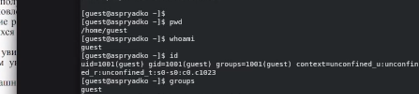
\includegraphics[keepaspectratio]{./image/user_info.png}}
\end{column}
\end{columns}
\end{frame}

\begin{frame}[fragile]{Исследование системных атрибутов}
\phantomsection\label{ux438ux441ux441ux43bux435ux434ux43eux432ux430ux43dux438ux435-ux441ux438ux441ux442ux435ux43cux43dux44bux445-ux430ux442ux440ux438ux431ux443ux442ux43eux432}
\begin{columns}[c]
\begin{column}{0.5\linewidth}
\begin{itemize}[<+->]
\tightlist
\item
  Изучена строка пользователя в \texttt{/etc/passwd}
\item
  Проверены права на домашние каталоги
\item
  Попытка просмотра расширенных атрибутов (\texttt{lsattr})
\end{itemize}
\end{column}

\begin{column}{0.5\linewidth}
\pandocbounded{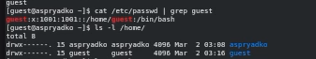
\includegraphics[keepaspectratio]{./image/system_files.png}}
\end{column}
\end{columns}
\end{frame}

\begin{frame}[fragile]{Эксперименты с правами (chmod 000)}
\phantomsection\label{ux44dux43aux441ux43fux435ux440ux438ux43cux435ux43dux442ux44b-ux441-ux43fux440ux430ux432ux430ux43cux438-chmod-000}
\begin{columns}[c]
\begin{column}{0.5\linewidth}
\begin{itemize}[<+->]
\tightlist
\item
  Создана папка \texttt{dir1}
\item
  Установлены права \texttt{000}
\item
  Зафиксирован полный отказ в доступе (Permission denied)
\end{itemize}
\end{column}

\begin{column}{0.5\linewidth}
\pandocbounded{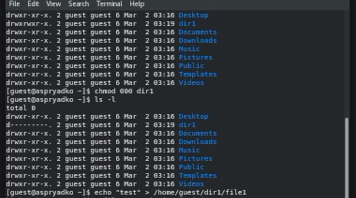
\includegraphics[keepaspectratio]{./image/dir_creation.png}}
\end{column}
\end{columns}
\end{frame}

\begin{frame}[fragile]{Ограничение доступа (chmod 100)}
\phantomsection\label{ux43eux433ux440ux430ux43dux438ux447ux435ux43dux438ux435-ux434ux43eux441ux442ux443ux43fux430-chmod-100}
\begin{columns}[c]
\begin{column}{0.5\linewidth}
\begin{itemize}[<+->]
\tightlist
\item
  Установка права \texttt{x} (выполнение) на папку
\item
  Результат: \texttt{cd} разрешен, но \texttt{ls} и
  \texttt{echo\ \textgreater{}} запрещены
\item
  Право \enquote{прохода} без права \enquote{чтения списка}
\end{itemize}
\end{column}

\begin{column}{0.5\linewidth}
\pandocbounded{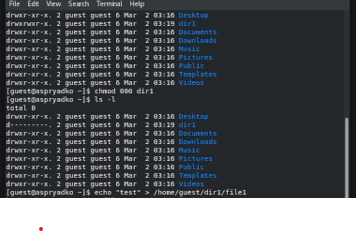
\includegraphics[keepaspectratio]{./image/denial_tests.png}}
\end{column}
\end{columns}
\end{frame}

\begin{frame}[fragile]{Анализ минимальных прав}
\phantomsection\label{ux430ux43dux430ux43bux438ux437-ux43cux438ux43dux438ux43cux430ux43bux44cux43dux44bux445-ux43fux440ux430ux432}
\begin{columns}[c]
\begin{column}{0.5\linewidth}
\begin{itemize}[<+->]
\tightlist
\item
  Чтение файла при \texttt{chmod\ 100} на папку (успешно)
\item
  Удаление файла при \texttt{chmod\ 000} на файл (успешно при
  \texttt{700} на папку)
\item
  Подтверждена роль прав родительской директории
\end{itemize}
\end{column}

\begin{column}{0.5\linewidth}
\pandocbounded{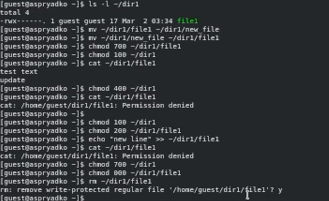
\includegraphics[keepaspectratio]{./image/minimal_rights_test.png}}
\end{column}
\end{columns}
\end{frame}

\section{Результаты}\label{ux440ux435ux437ux443ux43bux44cux442ux430ux442ux44b}

\begin{frame}{Установленные права и разрешённые действия}
\phantomsection\label{ux443ux441ux442ux430ux43dux43eux432ux43bux435ux43dux43dux44bux435-ux43fux440ux430ux432ux430-ux438-ux440ux430ux437ux440ux435ux448ux451ux43dux43dux44bux435-ux434ux435ux439ux441ux442ux432ux438ux44f}
\begin{longtable}[]{@{}
  >{\raggedright\arraybackslash}p{(\linewidth - 18\tabcolsep) * \real{0.0816}}
  >{\centering\arraybackslash}p{(\linewidth - 18\tabcolsep) * \real{0.1020}}
  >{\centering\arraybackslash}p{(\linewidth - 18\tabcolsep) * \real{0.1020}}
  >{\centering\arraybackslash}p{(\linewidth - 18\tabcolsep) * \real{0.1020}}
  >{\centering\arraybackslash}p{(\linewidth - 18\tabcolsep) * \real{0.1020}}
  >{\centering\arraybackslash}p{(\linewidth - 18\tabcolsep) * \real{0.1020}}
  >{\centering\arraybackslash}p{(\linewidth - 18\tabcolsep) * \real{0.1020}}
  >{\centering\arraybackslash}p{(\linewidth - 18\tabcolsep) * \real{0.1020}}
  >{\centering\arraybackslash}p{(\linewidth - 18\tabcolsep) * \real{0.1020}}
  >{\centering\arraybackslash}p{(\linewidth - 18\tabcolsep) * \real{0.1020}}@{}}
\toprule\noalign{}
\begin{minipage}[b]{\linewidth}\raggedright
Права дир.
\end{minipage} & \begin{minipage}[b]{\linewidth}\centering
Права файла
\end{minipage} & \begin{minipage}[b]{\linewidth}\centering
Созд.
\end{minipage} & \begin{minipage}[b]{\linewidth}\centering
Удал.
\end{minipage} & \begin{minipage}[b]{\linewidth}\centering
Запись
\end{minipage} & \begin{minipage}[b]{\linewidth}\centering
Чтение
\end{minipage} & \begin{minipage}[b]{\linewidth}\centering
cd
\end{minipage} & \begin{minipage}[b]{\linewidth}\centering
ls
\end{minipage} & \begin{minipage}[b]{\linewidth}\centering
Переим.
\end{minipage} & \begin{minipage}[b]{\linewidth}\centering
chmod
\end{minipage} \\
\midrule\noalign{}
\endhead
d (000) & 0 & - & - & - & - & - & - & - & - \\
d (100) & 0 & - & - & - & - & + & - & - & + \\
drwx (700) & -rwx (700) & + & + & + & + & + & + & + & + \\
\bottomrule\noalign{}
\end{longtable}
\end{frame}

\begin{frame}{Минимальные права для совершения операций}
\phantomsection\label{ux43cux438ux43dux438ux43cux430ux43bux44cux43dux44bux435-ux43fux440ux430ux432ux430-ux434ux43bux44f-ux441ux43eux432ux435ux440ux448ux435ux43dux438ux44f-ux43eux43fux435ux440ux430ux446ux438ux439}
\begin{longtable}[]{@{}lcc@{}}
\toprule\noalign{}
Операция & Права на директорию & Права на файл \\
\midrule\noalign{}
\endhead
Создание файла & wx (3) & --- \\
Удаление файла & wx (3) & --- \\
Чтение файла & x (1) & r (4) \\
Запись в файл & x (1) & w (2) \\
Переименование & wx (3) & --- \\
\bottomrule\noalign{}
\end{longtable}
\end{frame}

\section{Итоги}\label{ux438ux442ux43eux433ux438}

\begin{frame}[fragile]{Выводы}
\phantomsection\label{ux432ux44bux432ux43eux434ux44b}
\begin{itemize}[<+->]
\tightlist
\item
  Права на директорию определяют доступ к её содержимому
\item
  Атрибут \textbf{\texttt{x}} на папку необходим для обращения к файлам
  внутри неё
\item
  Удаление файла --- это операция изменения \textbf{директории} (требует
  \texttt{wx} на папку)
\item
  Права на сам файл при его удалении не имеют значения для владельца
  директории
\end{itemize}
\end{frame}

\begin{frame}{Финальный слайд}
\phantomsection\label{ux444ux438ux43dux430ux43bux44cux43dux44bux439-ux441ux43bux430ux439ux434}
\begin{itemize}[<+->]
\tightlist
\item
  Дискреционное управление доступом --- база безопасности Linux
\item
  \textbf{Спасибо за внимание!}
\end{itemize}
\end{frame}




\end{document}
